\documentclass[border=10pt]{standalone}

\usepackage{tikz}
\usepackage{tikzsymbols}
\usetikzlibrary{calc,patterns,shapes.geometric}

\def\centerarc[#1](#2)(#3:#4:#5){\draw[#1] ($(#2)+({#5*cos(#3)},{#5*sin(#3)})$) arc (#3:#4:#5);}

\begin{document}
	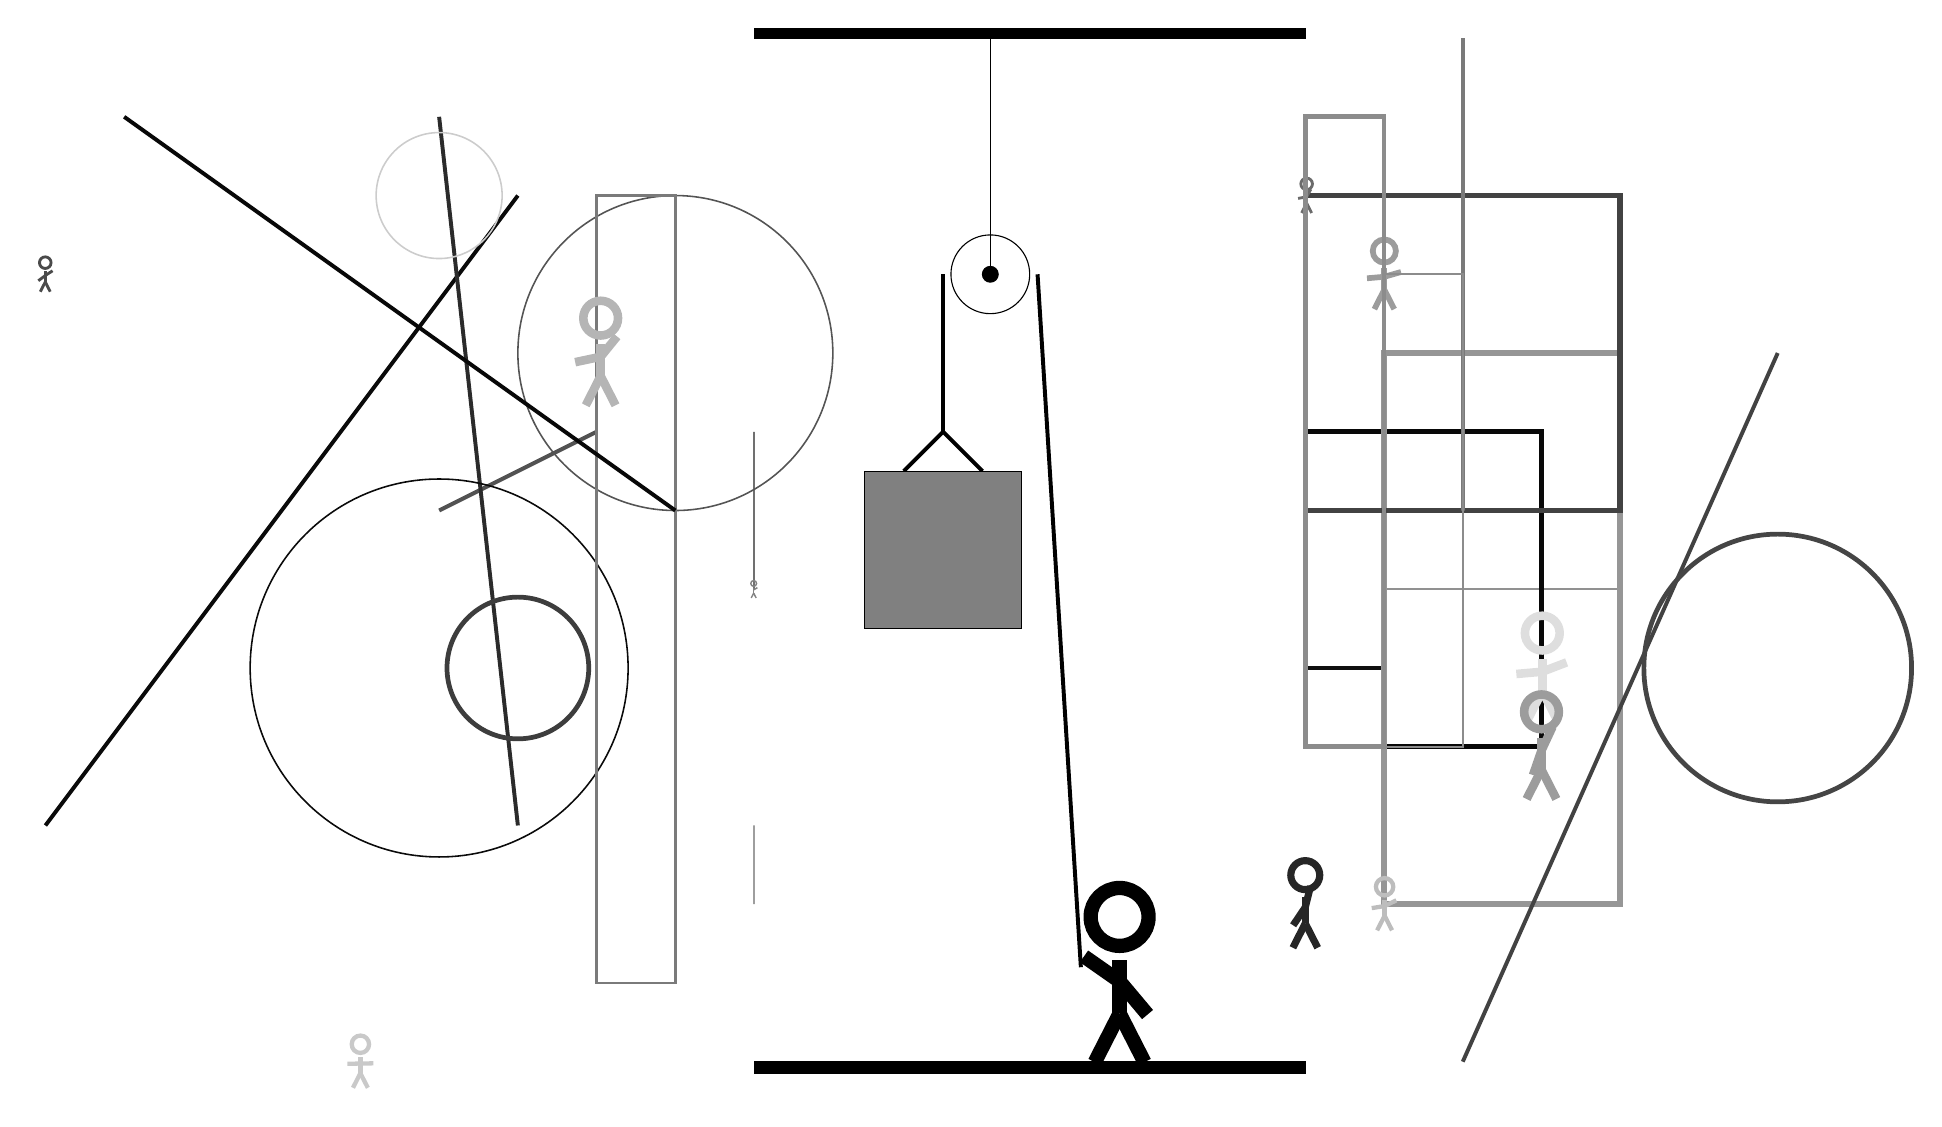
\begin{tikzpicture}
		%%%%% START %%%%%
		
		\draw[fill=black] (-2, 10) rectangle (5, 10.125);
		
		\draw (1, 7) circle (0.5);
		\draw[fill=black] (1, 7) circle (0.1);
		\draw (1, 10) -- (1, 7);
		
		\draw[line width=0.3mm, color=black!56] (-2, 3) rectangle (-2, 5);
		
		\draw[line width=0.5mm, color=black!68](-4, 5) -- (-6, 4);
		\node[line width=0.6mm, color=black!71] at (-11, 7) {\Strichmaxerl[2][37][33]};
		\draw[line width=0.3mm, color=black!43] (6, 3) rectangle (9, 4);
		\draw[line width=0.5mm, color=black!96](-5, 8) -- (-11, 0);
		
		\draw[line width=0.6mm, color=black!97] (5, 1) rectangle (8, 5);
		\draw[line width=0.5mm, color=black!83](-6, 9) -- (-5, 0);
		\draw[line width=0.5mm, color=black!94] (5, 2) rectangle (6, 4);
		\draw[line width=0.7mm, color=black!41] (6, -1) rectangle (9, 6);
		\draw[line width=0.7mm, color=black!74] (5, 8) rectangle (9, 4);
		\draw [line width=0.2mm, color=black!96](-6, 2) circle (2.4);
		
		\node[line width=0.4mm, color=black!26] at (6, -1) {\Strichmaxerl[3][9][26]};
		\node[line width=0.7mm, color=black!85] at (5, -1) {\Strichmaxerl[5][56][76]};
		
		\draw[line width=0.5mm, color=black!74](7, -3) -- (11, 6);
		\draw [line width=0.2mm, color=black!67](-3, 6) circle (2.0);
		\draw[line width=0.5mm, color=black!52] (7, 4) rectangle (7, 10);
		
		\node[line width=0.5mm, color=black!58] at (5, 8) {\Strichmaxerl[2][11][61]};
		
		\draw [line width=0.2mm, color=black!20](-6, 8) circle (0.8);
		\draw[line width=0.3mm, color=black!52] (-3, 8) rectangle (-4, -2);
		
		\node[line width=0.3mm, color=black!29] at (-4, 6) {\Strichmaxerl[6][12][51]};
		\node[line width=0.6mm, color=black!49] at (-2, 3) {\Strichmaxerl[1][90][31]};
		
		\draw [line width=0.6mm, color=black!73](11, 2) circle (1.7);
		
		\node[line width=0.3mm, color=black!13] at (8, 2) {\Strichmaxerl[6][5][21]};
		\draw[line width=0.3mm, color=black!38] (-2, 0) rectangle (-2, -1);
		\node[line width=0.7mm, color=black!39] at (8, 1) {\Strichmaxerl[6][71][65]};
		
		\node[line width=0.4mm, color=black!39] at (6, 7) {\Strichmaxerl[4][5][16]};
		\draw [line width=0.6mm, color=black!76](-5, 2) circle (0.9);
		\draw[line width=0.2mm, color=black!45] (6, 1) rectangle (7, 7);
		\node[line width=0.5mm, color=black!21] at (-7, -3) {\Strichmaxerl[3][1][1]};
		\draw[line width=0.5mm, color=black!97](-3, 4) -- (-10, 9);
		\draw[line width=0.6mm, color=black!45] (5, 1) rectangle (6, 9);
		
		\draw[line width=0.5mm] (-0.1, 4.5) -- (0.4, 5.0) -- (0.9, 4.5);
		\draw[fill=black!50] (-0.6, 4.5) rectangle (1.4, 2.5);
		
		\draw[line width=0.5mm] (0.4, 7) -- (0.4, 5.0);
		\centerarc[line width=0.5mm](1, 7)(0:180:0.6);
		\draw[line width=0.5mm](1.6, 7) -- (2.15, -1.8);
		
		\node at (2.6, -1.9) {\Strichmaxerl[10][-35][-50]};
		
		\draw[fill=black] (-2, -3) rectangle (5, -3.15);
		
		%%%%% END %%%%%
	\end{tikzpicture}
\end{document}